\chapter{Oxidatie en reductie}\label{ch:g11:redox}

Een zinken strip wordt in een blauwe oplossing van kopersulfaat
gedompeld. Binnen een paar minuten wordt het oppervlak donker onder een
sponzig, roodbruin laagje; een uur later is het blauw van de oplossing
verbleekt. Er is koper verschenen waar er geen was, en zink is als
onzichtbare \omterm{def:g9:ions:ion}{ionen} in oplossing gegaan. Er is niets verwarmd, er is geen
gas ontstaan, er deed geen zuurstof mee --- en toch noemen scheikundigen
dit een \omterm{def:g11:redox:oxidation}{oxidatie}. Het woord betekende vroeger ``zich verbinden met
zuurstof''; nu betekent het iets algemeners en nuttigers: het afstaan van
\omterm{def:g9:inside-the-atom:nucleus}{elektronen}. Dit hoofdstuk volgt de \omterm{def:g9:inside-the-atom:nucleus}{elektronen}.

\begin{recall}
Een \omterm{def:g9:ions:ion}{ion} is een \omterm{def:g7:atoms-and-molecules:atom}{atoom} of een groep \omterm{def:g7:atoms-and-molecules:atom}{atomen} die \omterm{def:g9:inside-the-atom:nucleus}{elektronen} heeft opgenomen
of afgestaan (\cref{ch:g9:ions}). Een \omterm{def:g9:periodic-table-first-look:metal}{metaal} zoals ijzer of zink reageert
met zoutzuur tot waterstof en metaalionen
(\cref{ch:g9:metals-acids-corrosion}). Een \omterm{def:g10:the-mole:amount}{hoeveelheid stof} $n$, in \omterm{def:g10:the-mole:amount}{mol},
bereken je uit een massa $m$ met $n = m/M$ (\cref{ch:g10:the-mole}).
\end{recall}

\begin{omfigure}
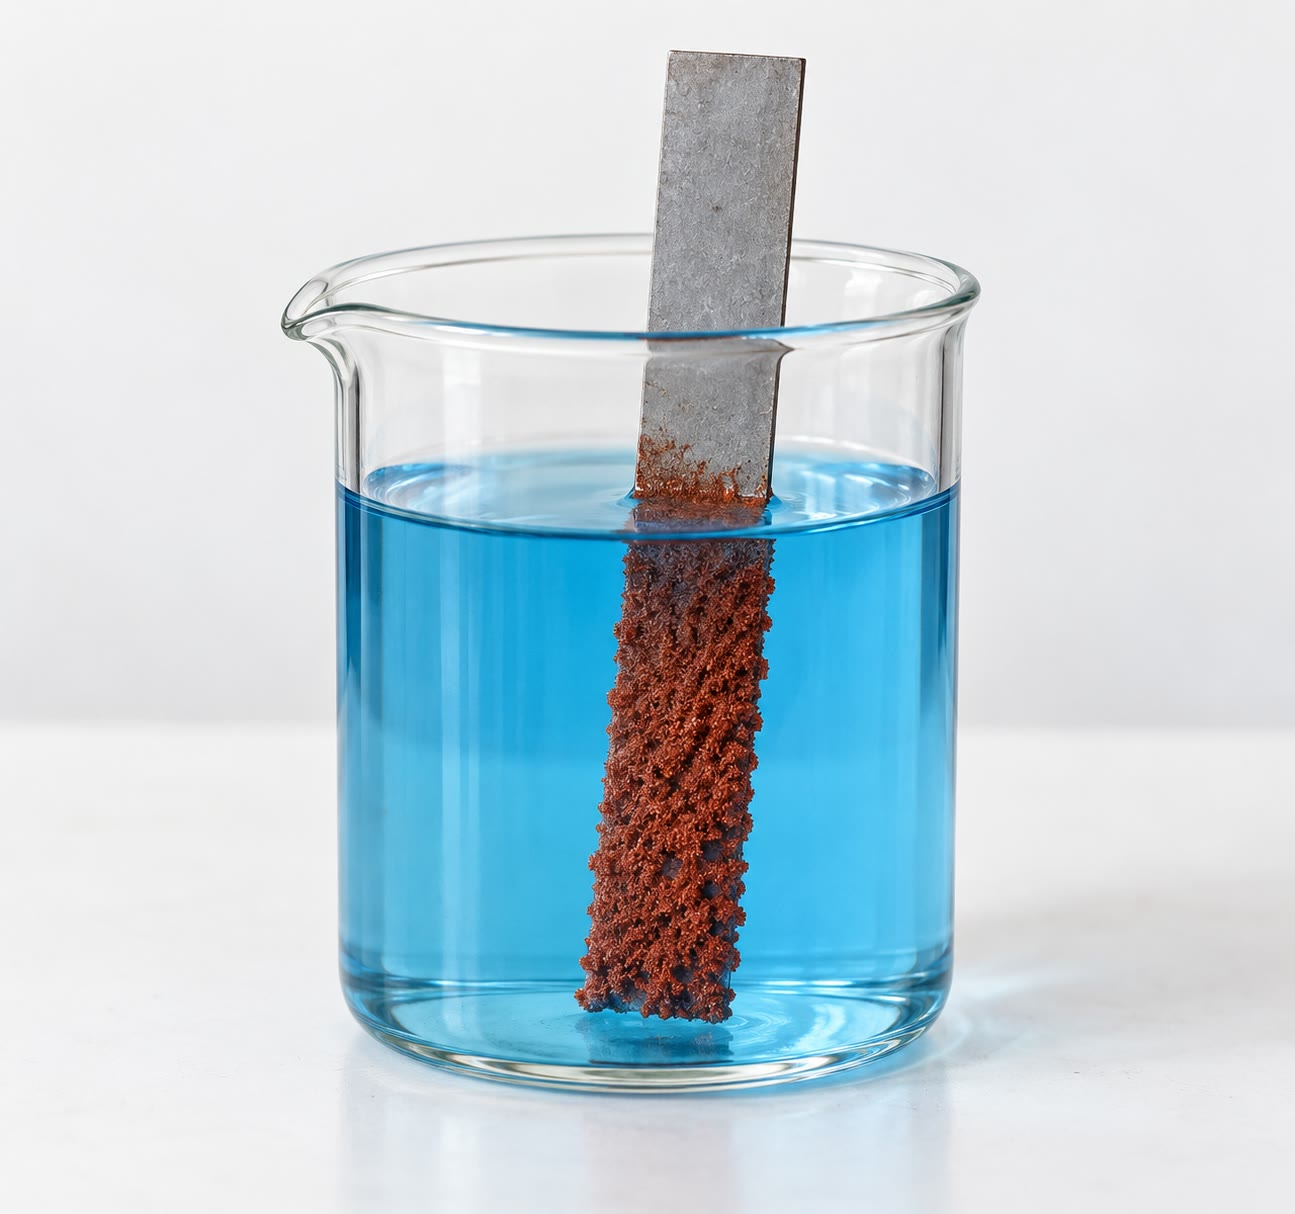
\includegraphics[width=0.55\linewidth]{images/book1/ai/g11-zinc-copper-sulfate.jpg}

{\small Een zinken strip in kopersulfaatoplossing: er slaat koper neer op
het zink, en zinkionen nemen zijn plaats in de oplossing in.}
\end{omfigure}

\section{Oxidatoren en reductoren}

\begin{definition}[Oxidator en reductor]\label{def:g11:redox:oxidant}
Een \emph{oxidator}\index{oxidator} is een deeltje dat een of meer
\omterm{def:g9:inside-the-atom:nucleus}{elektronen} kan opnemen. Een \emph{reductor}\index{reductor} is een
deeltje dat een of meer \omterm{def:g9:inside-the-atom:nucleus}{elektronen} kan afstaan.
\end{definition}

\begin{definition}[Oxidatie en reductie]\label{def:g11:redox:oxidation}
Een \emph{oxidatie}\index{oxidatie} is het afstaan van \omterm{def:g9:inside-the-atom:nucleus}{elektronen}; een
\emph{reductie}\index{reductie} is het opnemen van \omterm{def:g9:inside-the-atom:nucleus}{elektronen}. Een
\omterm{def:g11:redox:oxidant}{reductor} wordt geoxideerd; een \omterm{def:g11:redox:oxidant}{oxidator} wordt gereduceerd.
\end{definition}

\begin{remark}[Een ezelsbruggetje]\label{rem:g11:redox:remember}
Bij een \emph{\omterm{def:g11:redox:oxidation}{reductie}} wordt de lading van het deeltje verlaagd
(gereduceerd): \ce{Cu^{2+}} dat twee \omterm{def:g9:inside-the-atom:nucleus}{elektronen} opneemt, wordt \ce{Cu},
lading $+2 \to 0$. Bij een \omterm{def:g11:redox:oxidation}{oxidatie} gaat de lading omhoog:
\ce{Zn -> Zn^{2+} + 2e-}, $0 \to +2$.
\end{remark}

\begin{definition}[Redoxkoppel en halfreactie]\label{def:g11:redox:couple}
Een \omterm{def:g11:redox:oxidant}{oxidator} en de \omterm{def:g11:redox:oxidant}{reductor} die hij wordt door \omterm{def:g9:inside-the-atom:nucleus}{elektronen} op te nemen,
vormen een \emph{redoxkoppel}\index{redoxkoppel}, geschreven als Ox/Red
met de \omterm{def:g11:redox:oxidant}{oxidator} eerst: \ce{Cu^{2+}}/\ce{Cu}, \ce{Zn^{2+}}/\ce{Zn}. De
uitwisseling van \omterm{def:g9:inside-the-atom:nucleus}{elektronen} binnen een koppel wordt beschreven door de
\emph{halfreactie}\index{halfreactie},
\[
  \text{Ox} + n\,\ce{e-} \ce{<=>} \text{Red}, % ce-unbalanced-ok (generic form)
\]
kloppend in \omterm{def:g7:atoms-and-molecules:atom}{atomen} en in lading, bijvoorbeeld
$\ce{Cu^{2+}(aq) + 2e- <=> Cu(s)}$. De dubbele pijl zegt dat de
uitwisseling beide kanten op kan.
\end{definition}

\begin{example}[Metalen en hun ionen]\label{ex:g11:redox:metals}
Elk \omterm{def:g9:periodic-table-first-look:metal}{metaal} vormt een koppel met zijn \omterm{def:g9:ions:ion}{ion}:
\begin{center}
\begin{tabular}{ll}
\hline
koppel & \omterm{def:g11:redox:couple}{halfreactie} \\
\hline
\ce{Ag+}/\ce{Ag} & \ce{Ag+ + e- <=> Ag} \\
\ce{Cu^{2+}}/\ce{Cu} & \ce{Cu^{2+} + 2e- <=> Cu} \\
\ce{Fe^{2+}}/\ce{Fe} & \ce{Fe^{2+} + 2e- <=> Fe} \\
\ce{Zn^{2+}}/\ce{Zn} & \ce{Zn^{2+} + 2e- <=> Zn} \\
\ce{Al^{3+}}/\ce{Al} & \ce{Al^{3+} + 3e- <=> Al} \\
\hline
\end{tabular}
\end{center}
Ook \omterm{def:g9:ions:ion}{ionen} kunnen koppels vormen: \ce{Fe^{3+} + e- <=> Fe^{2+}} voor het
koppel \ce{Fe^{3+}}/\ce{Fe^{2+}}, en \ce{I2 + 2e- <=> 2I-} voor
\ce{I2}/\ce{I-}. Waterstof ook: \ce{2H+ + 2e- <=> H2} voor
\ce{H+}/\ce{H2}.
\end{example}

\begin{remark}[Eén deeltje, twee rollen]\label{rem:g11:redox:amphoteric}
Een deeltje kan de \omterm{def:g11:redox:oxidant}{reductor} van het ene koppel zijn en de \omterm{def:g11:redox:oxidant}{oxidator} van
een ander. Het \omterm{def:g9:ions:ion}{ion} \ce{Fe^{2+}} is de \omterm{def:g11:redox:oxidant}{oxidator} van \ce{Fe^{2+}}/\ce{Fe}
en de \omterm{def:g11:redox:oxidant}{reductor} van \ce{Fe^{3+}}/\ce{Fe^{2+}}. Welke rol het speelt,
hangt af van zijn partner in de reactie.
\end{remark}

\section{Redoxreacties}

\begin{definition}[Redoxreactie]\label{def:g11:redox:reaction}
Een \emph{redoxreactie}\index{redoxreactie} is een overdracht van
\omterm{def:g9:inside-the-atom:nucleus}{elektronen} van de \omterm{def:g11:redox:oxidant}{reductor} van het ene koppel naar de \omterm{def:g11:redox:oxidant}{oxidator} van een
ander. De \omterm{def:g11:redox:oxidant}{reductor} wordt geoxideerd en de \omterm{def:g11:redox:oxidant}{oxidator} wordt gereduceerd,
tegelijkertijd.
\end{definition}

\begin{proposition}[Geen vrije elektronen]\label{prop:g11:redox:no-free-electrons}
\omterm{def:g9:inside-the-atom:nucleus}{Elektronen} bestaan niet vrij in een oplossing: elk \omterm{def:g9:inside-the-atom:nucleus}{elektron} dat de
\omterm{def:g11:redox:oxidant}{reductor} afstaat, wordt door de \omterm{def:g11:redox:oxidant}{oxidator} opgenomen. De vergelijking van
een \omterm{def:g11:redox:reaction}{redoxreactie} krijg je daarom door de twee \omterm{def:g11:redox:couple}{halfreacties} op te tellen,
elk vermenigvuldigd met het getal dat de afgestane \omterm{def:g9:inside-the-atom:nucleus}{elektronen} gelijk
maakt aan de opgenomen \omterm{def:g9:inside-the-atom:nucleus}{elektronen}; de \omterm{def:g9:inside-the-atom:nucleus}{elektronen} vallen dan weg en komen
niet in de vergelijking voor.
\end{proposition}

\begin{example}[Zink en koperionen]\label{ex:g11:redox:zinc-copper}
In de openingsscène wordt het zink geoxideerd en worden de koperionen
gereduceerd:
\[
\begin{array}{l@{\qquad}l}
  \ce{Zn(s) -> Zn^{2+}(aq) + 2e-} & \text{(oxidatie)}\\
  \ce{Cu^{2+}(aq) + 2e- -> Cu(s)} & \text{(reductie)}\\
  \hline
  \ce{Zn(s) + Cu^{2+}(aq) -> Zn^{2+}(aq) + Cu(s)} &
\end{array}
\]
Van elk zinkatoom gaan twee \omterm{def:g9:inside-the-atom:nucleus}{elektronen} naar één koperion. De blauwe kleur
van de oplossing is de kleur van de \ce{Cu^{2+}}-ionen; die verbleekt
naarmate ze verbruikt worden, terwijl de kleurloze \ce{Zn^{2+}}-ionen hun
plaats innemen.
\end{example}

\begin{omfigure}
\begin{tikzpicture}[font=\small, >=Stealth,
    ion/.style={circle, draw=black!70, minimum size=10mm, inner sep=0pt}]
  % the zinc strip and the solution
  \fill[black!18] (0,0) rectangle (1.6,4);
  \draw[black!60] (1.6,0) -- (1.6,4);
  \node[anchor=south] at (0.8,0.08) {zink};
  \fill[omWater!60] (1.6,0) rectangle (9.0,4);
  \node[anchor=north east] at (8.95,3.95) {oplossing};
  % a zinc atom leaves as an ion
  \node[ion, fill=black!30] (zn) at (1.15,3.0) {\ce{Zn}};
  \node[ion, fill=white] (znion) at (5.0,3.0) {\ce{Zn^{2+}}};
  \draw[->, thick, omProp] (zn.east) -- (znion.west)
    node[midway, above] {oxidatie};
  % the electrons travel through the metal
  \draw[->, thick, omDef, dashed] (0.75,2.45) -- (0.75,1.55)
    node[midway, right] {2\,\ce{e-}};
  % a copper ion is reduced on the surface
  \node[ion, fill=omDef!35] (cuion) at (5.0,1.0) {\ce{Cu^{2+}}};
  \node[ion, fill=orange!55!brown] (cu) at (2.12,1.0) {\ce{Cu}};
  \draw[->, thick, omProp] (cuion.west) -- (cu.east)
    node[midway, above] {reductie};
  \node[anchor=west, align=left] at (6.1,2.0) {elk zinkatoom geeft\\ twee elektronen aan één\\ koperion};
\end{tikzpicture}

{\small Aan het oppervlak van het zink. Een zinkatoom staat twee
\omterm{def:g9:inside-the-atom:nucleus}{elektronen} af en vertrekt als \ce{Zn^{2+}}-ion; de twee \omterm{def:g9:inside-the-atom:nucleus}{elektronen} gaan
door het \omterm{def:g9:periodic-table-first-look:metal}{metaal} naar een \ce{Cu^{2+}}-ion dat het oppervlak raakt, en dat
wordt een koperatoom dat op de strip blijft zitten.}
\end{omfigure}

\begin{omfigure}
\begin{tikzpicture}[font=\small]
  \pic at (0,0) {beaker={0.75}{omDef!45}};
  \fill[black!35] (-0.15,0.25) rectangle (0.15,2.5);
  \draw[black!65] (-0.15,0.25) rectangle (0.15,2.5);
  \node[anchor=north, align=center] at (0,-0.15) {bij het begin:\\ blauwe \ce{Cu^{2+}}-oplossing};
  \draw[->, thick, omProp] (1.3,1) -- (3.2,1) node[midway, above] {één uur};
  \pic at (4.5,0) {beaker={0.75}{omDef!12}};
  \fill[black!35] (4.35,0.25) rectangle (4.65,2.5);
  \fill[orange!55!brown] (4.3,0.25) rectangle (4.7,1.5);
  \draw[black!65] (4.35,0.25) rectangle (4.65,2.5);
  \node[anchor=north, align=center] at (4.5,-0.15) {later: lichtere oplossing,\\ koper op het zink};
\end{tikzpicture}

{\small Wat je kunt zien: het koper dat neerslaat op het ondergedompelde
deel van de strip, en het verbleken van de blauwe kleur van de
\ce{Cu^{2+}}-ionen.}
\end{omfigure}

\begin{example}[Metalen in zuur, opnieuw bekeken]\label{ex:g11:redox:acid}
Als ijzer in zoutzuur \omterm{def:g2:mixing-and-dissolving:dissolve}{oplost}, wordt het ijzer geoxideerd en worden de
\ce{H+}-ionen gereduceerd tot waterstof:
\[
  \ce{Fe(s) + 2H+(aq) -> Fe^{2+}(aq) + H2(g)}.
\]
De koppels zijn \ce{Fe^{2+}}/\ce{Fe} en \ce{H+}/\ce{H2}; de
\omterm{def:g9:ions:ion}{chloride-ionen} doen niet mee.
\end{example}

\begin{inthelab}[De zilverboom]
Een spiraal van schoon koperdraad wordt in een bekerglas met verdunde
zilvernitraatoplossing gehangen, \ce{Ag+(aq) + NO3^-(aq)}. Binnen een uur
groeien er vertakte naalden glanzend zilver langs de draad, en de
kleurloze oplossing wordt lichtblauw:
\ce{Cu(s) + 2Ag+(aq) -> Cu^{2+}(aq) + 2Ag(s)}. Het experiment wordt door
de docent uitgevoerd, met handschoenen en veiligheidsbril, en de
oplossing wordt na afloop ingezameld als gevaarlijk afval.
\end{inthelab}

\begin{safety}{\ghs[0.82cm]{GHS03}\ghs[0.82cm]{GHS05}\ghs[0.82cm]{GHS08}\ghs[0.82cm]{GHS09}}
% ledger: ghs:AgNO3
Zilvernitraat: een oxiderende stof die een brand kan aanwakkeren
(GHS03); bijtend voor huid en ogen, en het kleurt de huid zwart (GHS05);
gevaarlijk voor de gezondheid (GHS08); zeer giftig voor in het water
levende organismen, dus het gaat nooit door de gootsteen (GHS09).
\end{safety}

\begin{omfigure}
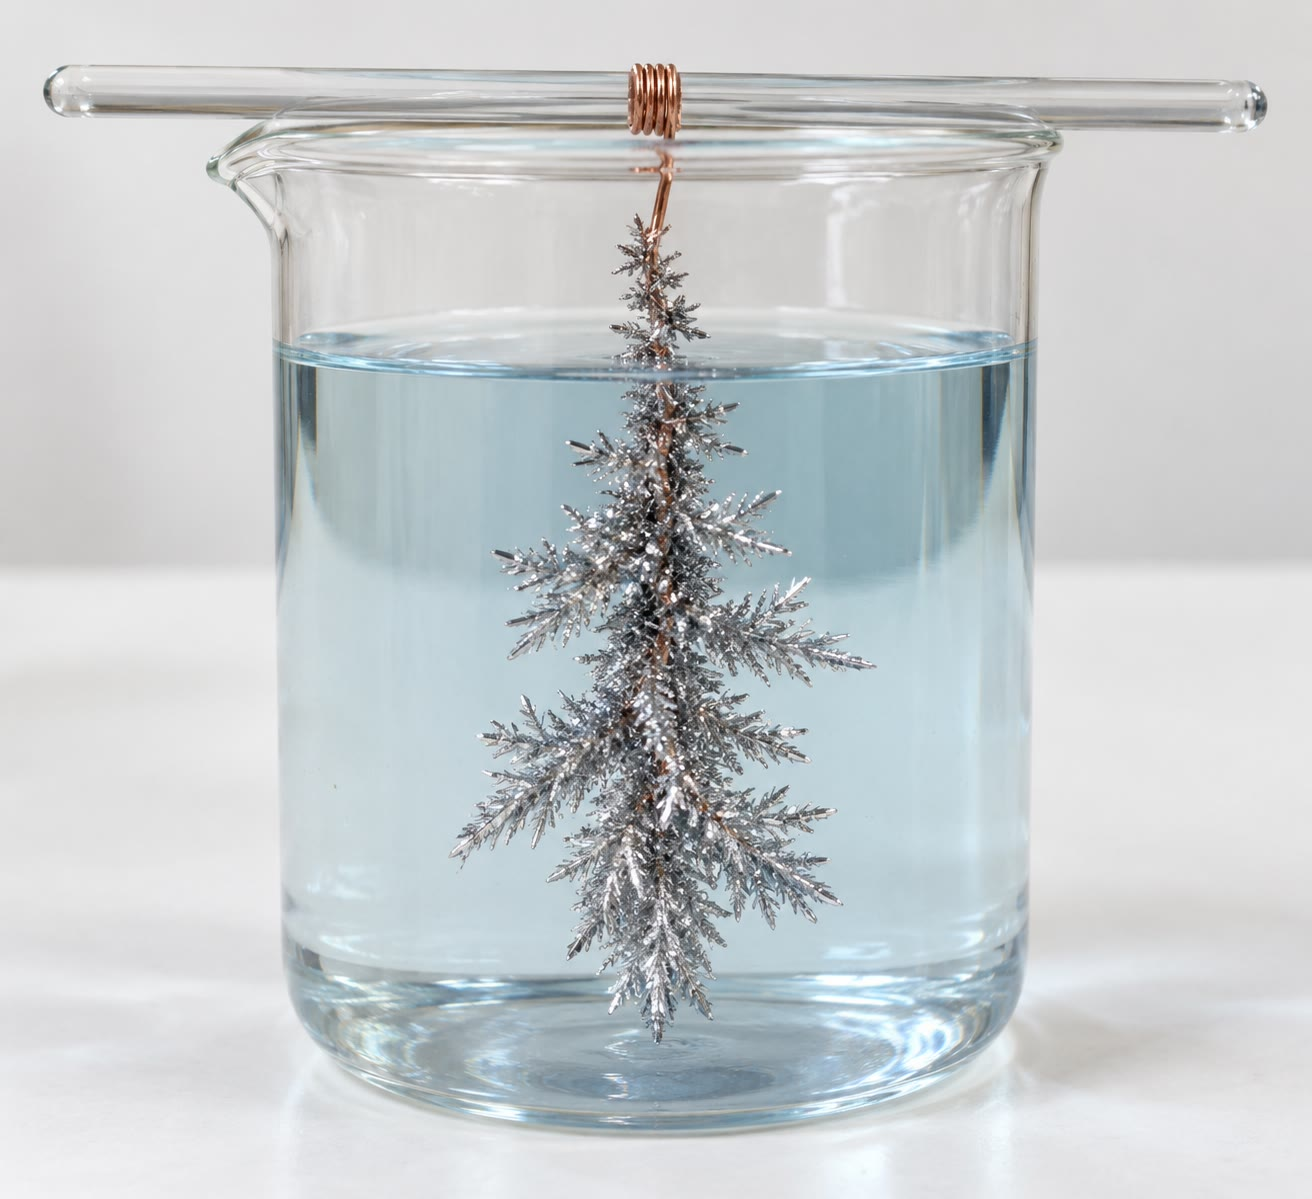
\includegraphics[width=0.5\linewidth]{images/book1/ai/g11-silver-tree.jpg}

{\small Zilverkristallen die groeien op een koperdraad in
zilvernitraatoplossing.}
\end{omfigure}

\section{Halfreacties kloppend maken}

Veel belangrijke koppels bevatten zuurstof en worden geschreven voor \omterm{def:g9:acids-bases-ph:acidic}{zure
oplossingen}, waarin \ce{H+}-ionen aanwezig zijn. Om hun \omterm{def:g11:redox:couple}{halfreacties}
kloppend te maken, zijn watermoleculen en \ce{H+}-ionen nodig.

\begin{method}[Een halfreactie in zure oplossing kloppend maken]\label{met:g11:redox:balance}
Zo schrijf je de \omterm{def:g11:redox:couple}{halfreactie} van een koppel Ox/Red in \omterm{def:g9:acids-bases-ph:acidic}{zure oplossing}:
\begin{enumerate}
  \item schrijf Ox links en Red rechts, en maak het \omterm{def:g7:atoms-and-molecules:atom}{atoom} kloppend dat
        geen O of H is;
  \item maak de zuurstofatomen kloppend met watermoleculen \ce{H2O};
  \item maak de waterstofatomen kloppend met \ce{H+}-ionen;
  \item maak de lading kloppend met \omterm{def:g9:inside-the-atom:nucleus}{elektronen} \ce{e-}, links;
  \item controleer: aan beide kanten evenveel \omterm{def:g7:atoms-and-molecules:atom}{atomen} van elke soort en
        dezelfde totale lading.
\end{enumerate}
\end{method}

\begin{example}[Het permanganaation]\label{ex:g11:redox:permanganate}
Voor het koppel \ce{MnO4^-}/\ce{Mn^{2+}} (dieppaars naar bijna
kleurloos): mangaan klopt; vier O links geven $\ce{4H2O}$ rechts; hun
acht H geven $\ce{8H+}$ links; de lading links is $-1 + 8 = +7$, rechts
$+2$, dus komen er links vijf \omterm{def:g9:inside-the-atom:nucleus}{elektronen} bij:
\[
  \ce{MnO4^-(aq) + 8H+(aq) + 5e- <=> Mn^{2+}(aq) + 4H2O(l)}.
\]
\end{example}

\begin{example}[Het dichromaation]\label{ex:g11:redox:dichromate}
Voor \ce{Cr2O7^{2-}}/\ce{Cr^{3+}} (oranje naar groen): twee chroom
rechts; zeven O geven \ce{7H2O}; veertien H geven \ce{14H+}; lading
$-2 + 14 = +12$ links tegen $2 \times 3 = +6$ rechts, dus zes
\omterm{def:g9:inside-the-atom:nucleus}{elektronen}:
\[
  \ce{Cr2O7^{2-}(aq) + 14H+(aq) + 6e- <=> 2Cr^{3+}(aq) + 7H2O(l)}.
\]
\end{example}

\begin{method}[Een redoxvergelijking opschrijven]\label{met:g11:redox:combine}
Zo schrijf je de vergelijking op van de reactie tussen de \omterm{def:g11:redox:oxidant}{oxidator} Ox$_1$
van het ene koppel en de \omterm{def:g11:redox:oxidant}{reductor} Red$_2$ van een ander:
\begin{enumerate}
  \item schrijf beide \omterm{def:g11:redox:couple}{halfreacties} op, de eerste in de richting van de
        \omterm{def:g11:redox:oxidation}{reductie} (Ox$_1 \to$ Red$_1$), de tweede in de richting van de
        \omterm{def:g11:redox:oxidation}{oxidatie} (Red$_2 \to$ Ox$_2$);
  \item vermenigvuldig ze met de kleinste getallen die de \omterm{def:g9:inside-the-atom:nucleus}{elektronen}
        gelijk maken;
  \item tel ze op; de \omterm{def:g9:inside-the-atom:nucleus}{elektronen} vallen weg, en soms ook \ce{H+} en
        \ce{H2O} die aan beide kanten staan;
  \item controleer \omterm{def:g7:atoms-and-molecules:atom}{atomen} en lading nog een keer.
\end{enumerate}
\end{method}

\begin{example}[Permanganaat en ijzer(II)]\label{ex:g11:redox:mno4-fe}
Het permanganaation oxideert \ce{Fe^{2+}}-ionen tot \ce{Fe^{3+}}:
\[
\begin{array}{l@{\qquad}l}
  \ce{MnO4^- + 8H+ + 5e- -> Mn^{2+} + 4H2O} & \times 1\\
  \ce{Fe^{2+} -> Fe^{3+} + e-} & \times 5\\
  \hline
  \ce{MnO4^- + 8H+ + 5Fe^{2+} -> Mn^{2+} + 5Fe^{3+} + 4H2O} &
\end{array}
\]
Lading links: $-1 + 8 + 10 = +17$; rechts: $2 + 15 = +17$. Deze reactie
wordt in het volgende hoofdstuk gebruikt om een hoeveelheid ijzer(II) te
meten.
\end{example}

\section{Oxidatoren en reductoren om ons heen}

\begin{proposition}[Enkele veelvoorkomende oxidatoren en reductoren]\label{prop:g11:redox:common}
De volgende deeltjes kom je in het laboratorium en in het dagelijks leven
steeds weer tegen:
\begin{center}
\small
\begin{tabular}{lll}
\hline
deeltje & rol & \omterm{def:g11:redox:couple}{halfreactie} van zijn koppel \\
\hline
zuurstof \ce{O2} & \omterm{def:g11:redox:oxidant}{oxidator} & \ce{O2 + 4H+ + 4e- <=> 2H2O} \\
chloor \ce{Cl2} & \omterm{def:g11:redox:oxidant}{oxidator} & \ce{Cl2 + 2e- <=> 2Cl-} \\
hypochloriet \ce{ClO-} (bleekwater) & \omterm{def:g11:redox:oxidant}{oxidator} & \ce{2ClO- + 4H+ + 2e- <=> Cl2 + 2H2O} \\
waterstofperoxide \ce{H2O2} & \omterm{def:g11:redox:oxidant}{oxidator} & \ce{H2O2 + 2H+ + 2e- <=> 2H2O} \\
permanganaat \ce{MnO4^-} & \omterm{def:g11:redox:oxidant}{oxidator} & \ce{MnO4^- + 8H+ + 5e- <=> Mn^{2+} + 4H2O} \\
\omterm{def:g9:periodic-table-first-look:metal}{metalen} \ce{M} (\ce{Fe}, \ce{Zn}, \ce{Al}\dots) & \omterm{def:g11:redox:oxidant}{reductoren} & \ce{M^{n+} + $n$ e- <=> M} % ce-unbalanced-ok (generic)
\\
jodide \ce{I-} & \omterm{def:g11:redox:oxidant}{reductor} & \ce{I2 + 2e- <=> 2I-} \\
thiosulfaat \ce{S2O3^{2-}} & \omterm{def:g11:redox:oxidant}{reductor} & \ce{S4O6^{2-} + 2e- <=> 2S2O3^{2-}} \\
ascorbinezuur \ce{C6H8O6} (vitamine C) & \omterm{def:g11:redox:oxidant}{reductor} & \ce{C6H6O6 + 2H+ + 2e- <=> C6H8O6} \\
\hline
\end{tabular}
\end{center}
\end{proposition}

\begin{example}[Koper wordt groen]\label{ex:g11:redox:patina}
Koperen daken en beelden die tientallen jaren buiten staan, worden
langzaam lichtgroen. Zuurstof uit de \omterm{def:g4:air-a-mixture-of-gases:air}{lucht} oxideert het koper tot
\ce{Cu^{2+}}-ionen, die met water en koolstofdioxide een dunne groene
korst vormen, de patina. Anders dan \omterm{def:g9:metals-acids-corrosion:corrosion}{roest} op ijzer hecht de patina aan
het \omterm{def:g9:periodic-table-first-look:metal}{metaal} en beschermt ze het tegen verdere aantasting.
\end{example}

\begin{omfigure}

\includegraphics[width=0.48\linewidth]{images/book1/ai/g11-green-roof.jpg}

{\small Een koperen dak na tientallen jaren aan de \omterm{def:g4:air-a-mixture-of-gases:air}{lucht}: geoxideerd
koper vormt een groene patina.}
\end{omfigure}

\begin{remark}[Antioxidanten]\label{rem:g11:redox:antioxidant}
Een ``antioxidant'' die aan voedsel wordt toegevoegd, is een \omterm{def:g11:redox:oxidant}{reductor} die
door de zuurstof van de \omterm{def:g4:air-a-mixture-of-gases:air}{lucht} geoxideerd wordt voordat het voedsel dat
wordt. Vitamine C (ascorbinezuur) is de bekendste: een doorgesneden
appel met wat citroensap erover wordt veel langzamer bruin, omdat eerst
de vitamine C van de citroen geoxideerd wordt.
\end{remark}

\section{Oefeningen}

\begin{exercise}[$\star$]\label{exo:g11:redox:1}
Definieer een \omterm{def:g11:redox:oxidant}{oxidator}, een \omterm{def:g11:redox:oxidant}{reductor}, een \omterm{def:g11:redox:oxidation}{oxidatie} en een \omterm{def:g11:redox:oxidation}{reductie}.
\end{exercise}

\begin{exercise}[$\star$]\label{exo:g11:redox:2}
Schrijf voor elk paar het \omterm{def:g11:redox:couple}{redoxkoppel} op in de vorm Ox/Red: \ce{Fe} en
\ce{Fe^{2+}}; \ce{Ag} en \ce{Ag+}; \ce{I-} en \ce{I2}; \ce{Fe^{2+}}
en \ce{Fe^{3+}}.
\end{exercise}

\begin{exercise}[$\star$]\label{exo:g11:redox:3}
Schrijf de \omterm{def:g11:redox:couple}{halfreacties} op van de koppels \ce{Ag+}/\ce{Ag},
\ce{Al^{3+}}/\ce{Al}, \ce{Fe^{3+}}/\ce{Fe^{2+}} en \ce{Cl2}/\ce{Cl-}.
\end{exercise}

\begin{exercise}[$\star$]\label{exo:g11:redox:4}
Is de omzetting \ce{Fe -> Fe^{2+} + 2e-} een \omterm{def:g11:redox:oxidation}{oxidatie} of een \omterm{def:g11:redox:oxidation}{reductie}?
Werkt ijzer hier als \omterm{def:g11:redox:oxidant}{oxidator} of als \omterm{def:g11:redox:oxidant}{reductor}?
\end{exercise}

\begin{exercise}[$\star$]\label{exo:g11:redox:5}
Noem in de reactie \ce{Zn + Cu^{2+} -> Zn^{2+} + Cu} het deeltje dat
geoxideerd wordt, het deeltje dat gereduceerd wordt, de \omterm{def:g11:redox:oxidant}{oxidator} en de
\omterm{def:g11:redox:oxidant}{reductor}, en geef het aantal \omterm{def:g9:inside-the-atom:nucleus}{elektronen} dat per zinkatoom wordt
overgedragen.
\end{exercise}

\begin{exercise}[$\star\star$]\label{exo:g11:redox:6}
Maak in \omterm{def:g9:acids-bases-ph:acidic}{zure oplossing} de \omterm{def:g11:redox:couple}{halfreactie} van het koppel \ce{H2O2}/\ce{H2O}
kloppend, en volg daarbij \cref{met:g11:redox:balance} stap voor
stap.
\end{exercise}

\begin{exercise}[$\star\star$]\label{exo:g11:redox:7}
Schrijf de vergelijking op van de reactie tussen jood \ce{I2} en het
thiosulfaation \ce{S2O3^{2-}}, die \omterm{def:g9:ions:ion}{jodide-ionen} en tetrathionaationen
\ce{S4O6^{2-}} oplevert.
\end{exercise}

\begin{exercise}[$\star\star$]\label{exo:g11:redox:8}
Schrijf de vergelijking van de zilverboomreactie op uit haar twee
\omterm{def:g11:redox:couple}{halfreacties}, en leg uit waarom de oplossing blauw wordt.
\end{exercise}

\begin{exercise}[$\star\star$]\label{exo:g11:redox:9}
Vitamine C, \ce{C6H8O6}, reageert met jood \ce{I2}. Schrijf de
vergelijking van de reactie op, en zeg welk deeltje de \omterm{def:g11:redox:oxidant}{reductor} is.
\end{exercise}

\begin{exercise}[$\star\star$]\label{exo:g11:redox:10}
Aluminium reageert met koper(II)\omterm{def:g9:ions:ion}{ionen}. Schrijf de vergelijking op, en leg
uit waarom de \omterm{def:g11:redox:couple}{halfreacties} met 2 en met 3 vermenigvuldigd moeten worden.
\end{exercise}

\begin{exercise}[$\star\star$]\label{exo:g11:redox:11}
Waterstofperoxide oxideert in \omterm{def:g9:acids-bases-ph:acidic}{zure oplossing} ijzer(II)\omterm{def:g9:ions:ion}{ionen} tot
ijzer(III)\omterm{def:g9:ions:ion}{ionen}. Schrijf de vergelijking op.
\end{exercise}

\begin{exercise}[$\star\star\star$]\label{exo:g11:redox:12}
Een zinken strip verliest \qty{1.30}{g} in een oplossing met een overmaat
koper(II)\omterm{def:g9:ions:ion}{ionen}. Hoeveel koper slaat er neer? Neem
$M(\ce{Zn}) = \qty{65.4}{g/mol}$ en $M(\ce{Cu}) = \qty{63.5}{g/mol}$.
\end{exercise}

\begin{exercise}[$\star\star\star$]\label{exo:g11:redox:13}
Schrijf de vergelijking op van de \omterm{def:g11:redox:oxidation}{oxidatie} van ijzer(II)\omterm{def:g9:ions:ion}{ionen} door
dichromaationen in \omterm{def:g9:acids-bases-ph:acidic}{zure oplossing}. Welke hoeveelheid \ce{Fe^{2+}} wordt
geoxideerd door \qty{0.010}{mol} dichromaationen?
\end{exercise}

\begin{exercise}[$\star\star\star$]\label{exo:g11:redox:14}
Bleekwater bevat hypochlorietionen \ce{ClO-} en \omterm{def:g9:ions:ion}{chloride-ionen}
\ce{Cl-}. Schrijf met de koppels \ce{ClO-}/\ce{Cl2} en \ce{Cl2}/\ce{Cl-}
de vergelijking op van de reactie die optreedt als bleekwater met een
zuur in aanraking komt, en leg uit waarom de etiketten van bleekwater en
van zure ontkalkers allebei waarschuwen dat je ze nooit mag \omterm{def:g2:mixing-and-dissolving:mix}{mengen}.
\end{exercise}

\begin{exercise}[$\star\star\star$]\label{exo:g11:redox:15}
In de figuur van het zinkoppervlak gaan de \omterm{def:g9:inside-the-atom:nucleus}{elektronen} door het \omterm{def:g9:periodic-table-first-look:metal}{metaal},
niet door de oplossing. Leg met \cref{prop:g11:redox:no-free-electrons}
uit waarom het koper op de zinken strip zelf neerslaat en niet ergens
anders in het bekerglas.
\end{exercise}

\section{Probleem: De blaastest}

\begin{problem}[{Weekendprobleem --- de chemie van een blaaspijpje: twee
koppels, een kleuromslag van oranje naar groen, de massa ethanol die een
pijpje kan aantonen, en de brandstofcel die het verving}]
\label{pb:g11:redox:1}
% ledger: ghs:K2Cr2O7, breath:ratio; molar masses from tools/molar_mass.py
% (0.1-rounded weights): K2Cr2O7 294.2, C2H6O 46.0 g/mol
De eerste blaastests op alcohol gebruikten een glazen buisje gevuld met
korrels silica, bedekt met oranje kaliumdichromaat, \ce{K2Cr2O7}, in
zuur. Ethanol, \ce{CH3CH2OH}, in de adem die door het buisje geblazen
wordt, reduceert de dichromaationen tot groene \ce{Cr^{3+}}-ionen en
wordt zelf geoxideerd tot ethaanzuur, \ce{CH3COOH}; de lengte van de
groene zone is een maat voor de ethanol. Stel dat een buisje
\qty{2.0}{mg} kaliumdichromaat bevat. Gebruik
$M(\ce{K}) = 39.1$, $M(\ce{Cr}) = 52.0$, $M(\ce{O}) = 16.0$,
$M(\ce{C}) = 12.0$, $M(\ce{H}) = \qty{1.0}{g/mol}$, $N_A =
\qty{6.02e23}{mol^{-1}}$ en $e = \qty{1.60e-19}{C}$.

\medskip
\noindent\textbf{Deel I --- Twee koppels.}
\begin{enumerate}
  \item Noem de twee \omterm{def:g11:redox:couple}{redoxkoppels} die meedoen, de \omterm{def:g11:redox:oxidant}{oxidator} eerst.
  \item Wordt ethanol geoxideerd of gereduceerd? Is het de \omterm{def:g11:redox:oxidant}{oxidator} of de
        \omterm{def:g11:redox:oxidant}{reductor}?
  \item Schrijf de \omterm{def:g11:redox:couple}{halfreactie} op van het koppel
        \ce{Cr2O7^{2-}}/\ce{Cr^{3+}} in \omterm{def:g9:acids-bases-ph:acidic}{zure oplossing}.
  \item Schrijf de \omterm{def:g11:redox:couple}{halfreactie} op van het koppel
        \ce{CH3COOH}/\ce{CH3CH2OH} in \omterm{def:g9:acids-bases-ph:acidic}{zure oplossing}.
  \item Leid daaruit de vergelijking van de reactie in het buisje af.
\end{enumerate}

\medskip
\noindent\textbf{Deel II --- Wat één buisje kan meten.}
\begin{enumerate}[resume]
  \item Verklaar de kleuromslag van de korrels.
  \item Bereken de \omterm{def:g10:the-mole:molar-mass}{molaire massa} van kaliumdichromaat.
  \item Bereken de hoeveelheid dichromaationen in het buisje.
  \item Welke hoeveelheid ethanol is er nodig om het hele buisje groen te
        maken?
  \item Leid daaruit de grootste massa ethanol af die één buisje kan
        meten.
\end{enumerate}

\medskip
\noindent\textbf{Deel III --- Van adem naar bloed.}
Iemand blaast \qty{1.0}{L} adem door het buisje; de groene zone groeit
evenredig met de massa ethanol die haar bereikt.
\begin{enumerate}[resume]
  \item De adem bevat \qty{0.25}{mg} ethanol per liter. Welk deel van het
        dichromaat wordt gebruikt?
  \item Het buisje is \qty{10}{cm} lang. Hoe lang is de groene zone?
  \item Ademanalysers gaan ervan uit dat \qty{2100}{L} adem evenveel
        ethanol bevat als \qty{1}{L} bloed. Schat de massa ethanol per
        liter bloed, in gram.
  \item Waarom begint de groene zone bij de inlaat van het buisje en
        groeit ze naar de uitlaat toe, in plaats van dat het hele buisje
        een beetje groen wordt?
  \item Waarom kun je een buisje maar één keer gebruiken?
\end{enumerate}

\medskip
\noindent\textbf{Deel IV --- De brandstofcel.}
Kaliumdichromaat draagt de pictogrammen
\ghs[0.6cm]{GHS03}\,\ghs[0.6cm]{GHS05}\,\ghs[0.6cm]{GHS06}\,\ghs[0.6cm]{GHS07}\,\ghs[0.6cm]{GHS08}\,\ghs[0.6cm]{GHS09}.
Moderne apparaten gebruiken in plaats daarvan een brandstofcel, waarin de
ethanol van de adem op een elektrode door zuurstof geoxideerd wordt, en
de vrijgekomen \omterm{def:g9:inside-the-atom:nucleus}{elektronen} door een draad stromen.
\begin{enumerate}[resume]
  \item Geef twee redenen, afgelezen uit de pictogrammen, waarom de
        dichromaatbuisjes zijn afgeschaft.
  \item Schrijf de vergelijking op van de \omterm{def:g11:redox:oxidation}{oxidatie} van ethanol door
        zuurstof, met het koppel \ce{O2}/\ce{H2O}.
  \item Hoeveel \omterm{def:g9:inside-the-atom:nucleus}{elektronen} staat één ethanolmolecuul af als het tot
        ethaanzuur geoxideerd wordt?
  \item Bereken voor \qty{0.25}{mg} ethanol de hoeveelheid ethanol, en
        daarna het aantal \omterm{def:g9:inside-the-atom:nucleus}{elektronen} dat vrijkomt.
  \item Leid daaruit de elektrische lading af die door de brandstofcel
        stroomt. Waarom is deze lading een goede maat voor de ethanol in
        de adem?
\end{enumerate}
\end{problem}
